\chapter{Quantum Systems}
\label{ch:impl_quantum_systems}

In order to study a quantum system on the computer it is necessary to 
make a distinction for what defines the system, and one must therefore undergo the
mathematical procedure of constructing a finite basis sets that defines the system in 
question. Here we present the \lstinline{quantum_systems} python module, mainly designed to 
provide basis sets for one- and two-dimensional quantum dots.

For the one-dimensional quantum dot we provide a wide selection of different
potentials. This is possible due to the relative computational ease associated with the 
model. As for the two-dimensional 
systems we have implemented each confining potential in separate classes including
the regular harmonic quantum dot, a 
double quantum dot, as well as a quantum dot affected by a homogenous, static  magnetic 
field.

In order to achieve maximum usability, the \lstinline{quantum_systems} module
includes a class for constructing custom systems, using basis sets imported from 
somwhere else, or basis sets defined by the user.
We have written functions that interface with popular quantum chemistry packages
\lstinline{PySCF}\cite{PYSCF} 
and \lstinline{Psi4}\cite{parrish2017psi4},
allowing the user to easily construct basis sets 
representing all kinds of systems of interest in quantum chemistry, like atoms and 
molecules. 

What is more, the \lstinline{quantum_systems} module also contains an implementation of 
a plane wave or homogenous electron gas basis set, sometimes called the 
jellium 
model\footnote{See for instance Ch. 10 in Gross and Heinonen \cite{gross1986many}}.
However, this implementation exists mainly as 
a curiosity at the time of writing. In the future it can potentially
be developed into something more useful,
as the electron gas can serve as a first approximation to a metal or a semi-conductor.

A complete diagrammatic class hierarchy of the \lstinline{quantum_systems} module 
can be found in \autoref{app:class_diagram}. This class hierarchy also illustrates how 
the \lstinline{quantum_systems} modules fits into and works with the 
\lstinline{coupled_cluster} module, to be presented in the next chapter.

The \lstinline{quantum_system} module can be installed from github with \lstinline{pip}
by the following command,
\begin{lstlisting}[language=bash]
pip install git+https://github.com/Schoyen/quantum-systems.git
\end{lstlisting}
The same task can of course be accomplished by more commands,
\begin{lstlisting}[language=bash]
git clone https://github.com/Schoyen/quantum-systems.git
cd quantum-systems
pip install .
\end{lstlisting}

It can be useful to install the module to a separate environment. We have made this 
possible through \lstinline{conda},
\begin{lstlisting}[language=bash]
conda environment create -f environment.yml
conda activate quantum-systems    
\end{lstlisting}

\section{Quantum System Abstract Base Class} 

Here we present the abstract base class that every system class in the
\lstinline{quantum_systems} module is built upon. This base class forms the foundation 
of any quantum system, in order to make a system specification work together with 
solver from the \lstinline{coupled_cluster} module presented in the next chapter. The base class is 
named \lstinline{QuantumSystem}.

\begin{figure}[h]
\begin{tcolorbox}
    {\fontfamily{cmss}\selectfont
    \textbf{class} quantum\_systems.\textbf{QuantumSystem}
    (\emph{n}, \emph{l}, \emph{n\_up=None}, \emph{np=None})

    \vspace{1em}
    Abstract base class defining the common methods used by all different quantum systems.

    \vspace{1em}
    \textbf{Parameters:} 

    \hspace{2em} \textbf{n} (\emph{int}) Number of electrons
    
    \hspace{2em} \textbf{l} (\emph{int}) Number of spinorbitals

    \hspace{2em} \textbf{n\_up} (\emph{int, default=None}) Number of spin-up spinorbitals

    \hspace{2em} \textbf{np} (\emph{module}) Matrix library, i.e. numpy, cupy etc.

    \vspace{1em}
    \textbf{Attributes:}

    \hspace{2em} \textbf{h}
    One-body matrix 
    \textbf{Type} \emph{np.array}
    
    \hspace{2em} \textbf{f}
    Fock matrix
    \textbf{Type} \emph{np.array}

    \hspace{2em} \textbf{u}
    Two-body matrix
    \textbf{Type} \emph{np.array}

    \hspace{2em} \textbf{s}
    Overlap matrix of spinorbitals
    \textbf{Type} \emph{np.array}
    
    \hspace{2em} \textbf{spf}
    Single-particle functions
    \textbf{Type} \emph{np.array}

    \hspace{2em} \textbf{spf\_bra}
    Conjugated single-particle functions
    \textbf{Type} \emph{np.array}

    % \hspace{2em} \textbf{o}
    % Occupied orbital indices
    % \textbf{Type} \emph{Slice} object

    % \hspace{2em} \textbf{v}
    % Virtual orbital indices
    % \textbf{Type} \emph{Slice} object

    \vspace{1em}
    \textbf{Methods:}

    \hspace{2em} \textbf{setup\_system}()
    \begin{adjustwidth}{4em}{}
        Method must be implemented by subclasses.
    \end{adjustwidth}

    \hspace{2em} \textbf{change\_basis}(\emph{c}, \emph{c\_tilde=None})
    \begin{adjustwidth}{4em}{}
        Changes basis of system according to coefficient matrices $\vb{C}$
        and $\tilde{\vb{C}}$.
    \end{adjustwidth}

    \hspace{2em} \textbf{change\_to\_hf\_basis}(\emph{*args}, \emph{verbose=False} \emph{**kwargs})
    \begin{adjustwidth}{4em}{}
        Changes basis of system to Hartree-Fock basis.
    \end{adjustwidth}

    \hspace{2em} \textbf{set\_time\_evolution\_operator}(\emph{time\_evolution\_operator})
    \begin{adjustwidth}{4em}{}
        Setter for time-evolution operator.

        \textbf{Parameters:} 
        
        \hspace{1.5em} \textbf{time\_evolution\_operator} (\emph{TimeEvolutionOperator}) 

    \end{adjustwidth}

    }
\end{tcolorbox}
\end{figure}

Many of the methods necessary to set up a quantum system can be abstracted away, which 
is most of the motivation for constructing a parent class that all other 
quantum system classes can inherit from. Examples of such functionality is 
setting up the Fock matrix. The one- and two-body operators are necessary to set up 
for a specific system, but the Fock matrix computations can be abstracted away 
to the superclass.

In the \lstinline{QuantumSystem} abstract base class we have included a
method that changes the basis of the system according to the coefficient matrices 
$\vb{C}$ and $\tilde{\vb{C}}$, the \lstinline{change_basis(...)} method.
This method will be useful later, especially when 
computing the basis for the double well system. In the time-dependent coupled cluster 
scheme with adaptive oribtals, this method becomes particularly useful. 

A similar method \lstinline{change_to_hf_basis()} is also implemented in the 
\lstinline{QuantumSystems} class. This changes the system basis to a basis based 
on the coefficient matrix found from the Roothan-Hall equations,
\begin{equation}
    FC = SC\epsilon,
\end{equation}
which are thoroughly discussed in \autoref{sec:roothan_hall_eqns}.
The basis transformation is performed by multiplication with the coefficient matrix,
\begin{equation}
    \ket{\phi_p} = C^\alpha_p \ket{\chi_\alpha},
\end{equation}
where we go from a (naïve) basis $\ket{\chi_\alpha}$, to the much better Hartree-Fock basis 
$\ket{\phi_p}$. The basis would be better suited to represent the system because it 
already consitutes an approximate ground state solution. The improvement in ground state 
energies by using the Hartree-Fock basis is well
documented\cite{jorgensen2011many,lohne2010coupled}.

The principal method that needs to be implemented in a subclass of
\lstinline{QuantumSystem} is
\lstinline{setup_system()}, including special considerations for dipole computations.
These factors will be discussed for each specific system we have implemented in the 
following sections.

\section{Quantum Dots}

In reality, quantum dots are nanometre-sized structures made of semiconductor materials.
Theoretically, quantum dots are easy to model with the harmonic oscillator potential and 
in practice
they are relatively easy to manufacture in a laboratory. This doubly
theoretical-experimental benefit has made quantum dots a popular area of study. Moreover so 
because of their wide area of applications.

The possible applications of quantum dots are many. Coupled single-electron quantum dots 
could potentially be used as hardware elements in quantum computers \cite{loss1998quantum}; quantum dots also promise to increase the efficiency of 
photovoltaic solar cells; and they have already found use in cellular imaging in biology.
Reimann and Manninen \cite{reimann2002electronic} has written a
thorough review on quantum dots, covering their varied types of fabrication, theoretical
methods common in their study and several applications.

We find that the study of quantum dot systems is warranted because of their great usefulness.
What is more, it is relatively easy to approximate such systems theoretically and 
numerically. 
Several classes have been implemented in the \lstinline{quantum_systems} module
that constructs basis sets modelling 
quantum dots in both one and two dimensions. Most of these basis sets model \emph{bound} systems
with the characteristics of infinite quantum wells. 

\subsection{One Dimension}

The one-dimensional quantum harmonic oscillator is perhaps one of the simplest of
all quantum mechanical models. It is studied thoroughly in every introductory quantum 
mechanics course. This is with good reason because the system is analytically easy to
manage, and because 
any arbitrary potential can be approxiamted by a harmonic oscillator as long 
as the oscillations are small enough.
One must bear in 
mind that the harmonic oscillator potential, sometimes also called the parabolic potential, 
is one of many potentials that one can use in a quantum dot system.

We have implemented 
the one-dimensional quantum dot in a class \lstinline{ODQD}, which is a subclass of 
the \lstinline{QuantumSystems} class. We will now go through some of the intricacies 
necessary to compute the basis set contained in the \lstinline{ODQD} class. Not much is 
needed, only a matrix representation of the one-body operator $\hat{h}$ and the two-body 
operator $\hat{u}$. In addition we need the single-particle functions, which are the 
eigenfunctions of $\hat{h}$.

The one-body part of the Hamiltonian for the one-dimensional quantum 
dot is,
\begin{equation}
    \label{eq:1d_ho_hamiltonian}
    \hat{h} = \hat{t} + \hat{v} = \frac{\hat{p}^2}{2m} + \frac{1}{2}m \omega^2\hat{x}^2,
\end{equation}
where the potential, $\hat{v} = \frac{1}{2}m \omega^2\hat{x}^2$, forms the well known 
harmonic potential, making this example implementation a harmonic quantum dot.
In a general one-dimensional system, this potential could 
readily be exchanged for something else. For instance that of the 
\emph{double well},
\begin{equation}
    \hat{v} = \frac{1}{2} m \omega^2
        \left(\hat{x}^2 + \frac{1}{4}l^2 - l |\hat{x}|\right),
\end{equation}
where $l$ is the width of a barrier in the middle of the parabolic 
potential. We have implemented several other potentials, which we summarise 
in \autoref{sec:1d_potentials}.

In atomic units we can set $\hbar = m = 1$. Substituting into the 
momentum operator, $\hat{p} = \hat{-i\hbar (\partial / \partial x)}$, this gives us 
\begin{equation}
    \label{eq:1d_hamiltonian}
    \hat{h} = - \frac{1}{2} \frac{\partial^2}{\partial x^2} + \hat{v}.
\end{equation}
The second-order derivative can be approximated by the central difference 
formula for some function $f(x)$, yielding
\begin{equation}
    f''(x) = \frac{f(x + dx) - 2f(x) +f(x - dx)}{dx^2},
\end{equation}
for some small $dx$. This means that we approximate the Hamilton 
operator of the system (\autoref{eq:1d_hamiltonian}) by a matrix,
\begin{equation}
    h^p_q =  \begin{pmatrix}
    1/dx^2 + v_1 & -1/2dx^2 & \ddots & & & \\
    -1/2dx^2 & 1/dx^2 + v_2 & -1/2dx^2 & \ddots & & \\
    \ddots & -1/2dx^2 & 1/dx^2 + v_3 & -1/2dx^2 & \ddots & \\
    & \ddots & \ddots & \ddots & \ddots & \ddots \\
    & & \ddots & -1/2dx^2 & 1/dx^2 + v_{n-1} & -1/2dx^2 \\
    & & & \ddots & -1/2dx^2 & 1/dx^2 + v_n
    \end{pmatrix},
\end{equation}
and we have thus transformed the time-independent Schrödinger equation
\begin{equation}
    \hat{h} \ket{\phi} = \epsilon \ket{\phi},
\end{equation}
into a matrix equation which constitutes a better representation on 
a computer. Here $n$ is 
the number of points used to numerically represent the wavefunction 
and Hamiltonian matrix representation. This is done with some generic 
eigenvalue solver, for instance \lstinline{numpy.linalg.eigh(...)}.
The eigenfunctions $\ket{\phi}$ provide the foundation for the single-particle functions
we need.

Since we would like to model interactions between particles we need something more
than just a numerical representation of the one-body operator. We therefore need to 
compute Coulomb integrals. 
The Coulomb integral matrix elements $u^{pq}_{rs}$ is computed in
several steps, starting with an ``inner intergral'' over all all space 
and two and two single-particle functions,
\begin{equation}
   u^q_s = \int \phi_q(x_1) \frac{\alpha}{(x_1-x_2)^2 + a^2}  \phi_s(x_2) dx,
\end{equation}
where $\alpha$ is the interaction strength parameter and $a$ is called the shielding 
parameter and is necessary for this integral 
to be calculable, as it avoids singular values in the integrand at $x_1=x_2$.
Numerically, this part is divided into two functions in our python implementation,
\begin{python}
def _shielded_coulomb(x_1, x_2, alpha, a):
    return alpha / np.sqrt((x_1 - x_2) ** + a ** 2)

def _compute_inner_integral(spf, l, num_grid_points, grid, alpha, a):
    inner_integral = np.zeros((l, l, num_grid_points), dtype=np.complex128)

    for q in range(l):
        for s in range(l):
            for i in range(num_grid_points):
                inner_integral[q, s, i] = _trapz(
                    spf[q]
                    * _shielded_coulomb(grid[i], grid, alpha, a)
                    * spf[s],
                    grid)

    return inner_integral
\end{python}

The inner orbital is subsequently used in the computation of the orbital integral,
\begin{equation}
    u^{pq}_{rs} = \int \phi_p u^q_s \phi_r dx,
\end{equation}
which is implemented numerically as follows,
\begin{python}
def _compute_orbital_integrals(spf, l, inner_integral, grid):
    u = np.zeros((l, l, l, l), dtype=np.complex128)

    for p in range(l):
        for q in range(l):
            for r in range(l):
                for s in range(l):
                    u[p, q, r, s] = _trapz(
                        spf[p] * inner_integral[q, s] * spf[r], grid)

    return u
\end{python}
Each integral is solved by the trapezoidal scheme, which approximates the integral 
by 
\begin{equation}
    \int_x^{x + \Delta x} f(x) dx \approx \Delta x \frac{f(x + \Delta x) - f(x)}{2}.
\end{equation}

Needless to say, computing the Coulomb integrals is one of the more intensive tasks,
and we therefore make great use of one the fly compilation from the 
\lstinline{numba} \cite{numba} module for Python.

\begin{figure}
\begin{tcolorbox}
    {\fontfamily{cmss}\selectfont
    \textbf{class} quantum\_systems.\textbf{ODQD}

    \hspace{1em}(\emph{n}, \emph{l}, \emph{grid\_length}, \emph{num\_grid\_points}, 
    \emph{a=$0.25$}, \emph{alpha=$1.0$})

    \vspace{1em}
    Create One-Dimensional Quantum Dot basis set.
    \vspace{1em}

    \textbf{Parameters}

    \hspace{2em}\textbf{n}(\emph{int}) Number of electrons
    
    \hspace{2em}\textbf{l}(\emph{int}) Number of spinorbitals
    
    \hspace{2em}\textbf{grid\_length}(\emph{int, float}) Space over which to 
        construct wavefunction.
    
    \hspace{2em}\textbf{num\_grid\_points}(\emph{int, float}) Number of 
        points for construction of wavefunction.

    \hspace{2em}\textbf{a}(\emph{float, default $0.25$}) Coulomb screening parameter.
    
    \hspace{2em}\textbf{alpha}(\emph{float, default $1.0$}) Coulomb strength parameter. 

    \vspace{1em}
    \textbf{Attributes}

    \hspace{2em} \textbf{h}
    One-body matrix 
    \textbf{Type} \emph{np.array}
    
    \hspace{2em} \textbf{f}
    Fock matrix
    \textbf{Type} \emph{np.array}

    \hspace{2em} \textbf{u}
    Two-body matrix
    \textbf{Type} np.array

    % \hspace{2em} \textbf{o}
    % Occupied orbital indices
    % \textbf{Type} \emph{Slice} object

    % \hspace{2em} \textbf{v}
    % Virtual orbital indices
    % \textbf{Type} \emph{Slice} object

    \vspace{1em}
    \textbf{Methods}

    \hspace{2em} \textbf{setup\_system}(\emph{Potential=None})
        \begin{adjustwidth}{4em}{}
        Must be called in order to compute basis functions. The method will 
        revert to regular harmonic oscillator potential with $\omega=0.25$
        if no potential has been provided.
        Optional potentials include one-dimensional double well potentials.           
        \end{adjustwidth}
   
    \hspace{2em} \textbf{contruct\_dipole\_moment}()
        \begin{adjustwidth}{4em}{}
        Constructs dipole moment. This method is called by
        \textbf{setup\_system}(). Necessary when constructing custom systems with 
        time development.
        \end{adjustwidth}
    }
\end{tcolorbox}

\end{figure}

\subsubsection{One-dimensional potentials}
\label{sec:1d_potentials}

We provide several one-dimensional potential classes (\autoref{tab:1d_potentials})
that can be passed to 
the \lstinline{setup_system(Potential)} method in the \lstinline{ODQD} class.
All these potentials are implemented as subclasses of the abstract 
base class \lstinline{OneDimPotential}. The only thing necessary for an 
inheriting class to implement is the primitive \lstinline{__call__} method which 
takes position on the grid, $x$, as argument, and must return 
the value of the potential at that point $x$.

The parabolic harmonic oscillator potential,
which we have made most use of and which is 
discussed above is implemented as follows,
\begin{python}
class HOPotential(OneDimPotential):
    def __init__(self, omega):
        self.omega = omega

    def __call__(self, x):
        return 0.5 * self.omega ** 2 * x ** 2
\end{python}

\begin{table}
    \caption{One-dimensional potential classes in \lstinline{quantum_systems}.}
    \centering
    \begin{tabular}{l c}
        \\
        \hline\hline \\ 
        \lstinline[]$DWPotential$         & 
        $\frac{1}{2}\omega^2\left(x^2 + \frac{1}{4}l^2 - l|x| \right)$ \\ [1em]
        \lstinline[]$DWPotentialSmooth$   &
        $\frac{1}{2a^2}\left(x + \frac{a}{2}\right)^2\left(x - \frac{a}{2}\right)^2$ \\ [1em]
        \lstinline[]$GaussianPotential$   &
        $Ae^{-\frac{(x-\mu)^2}{2\sigma^2}}$ \\ [1em]
        \lstinline[]$AtomicPotential$     &
        $- \frac{Z_a}{\sqrt{x^2 + c}}$ \\ [1em] \hline\hline
    \end{tabular} 
    \label{tab:1d_potentials}
\end{table}

\subsection{Two Dimensions}

The one-body part of the Hamiltonian for a two-dimensional quantum dots is almost
identical to the one-body part for a one-dimensional quantum dot. In cartesian
coordinates we merely include a second coordinate $y$ in the potential as well as
an $x$, but 
because we have analytical expressions for the Coulomb integrals in polar
coordinates\cite{anisimovas1998energy}, we write the one-body operator in 
polar coordinates as well,
\begin{equation}
    \label{eq:2d_ho_one_body_hamiltonian}
    \hat{h} = \frac{\hat{p}^2}{2m} + \frac{1}{2}m\omega^2\hat{r}^2
        = - \frac{\hbar^2}{2m}\left(
            \frac{\partial^2}{\partial r^2}
            + \frac{1}{r} \frac{\partial}{\partial r}
            + \frac{1}{r^2} \frac{\partial^2}{\partial \theta^2}
        \right)
        + \frac{1}{2}m\omega^2\hat{r}^2.
\end{equation}
The wavefunctions for a two-dimensional harmonic oscillator can be
written using the spherical harmonics,
\begin{equation}
    \label{eq:2d_ho_eigenstate}
    \phi(r,\theta) = N_{nm} R_{nm}(r) Y_m(\theta) = N_{nm} (ar)^{\abs{m}} L_n^{\abs{m}}(a^2r^2)
        e^{-a^2r^2/2} e^{im\theta},
\end{equation}
where $a=\sqrt{m\omega/\hbar}$ si the Bohr radius, $L^{\abs{m}}_n$ is 
the associated Laguerre polynomials, $n$ and $m$ are the principal and
the azimutal quantum numbers respectively\footnote{There is usually another quantum 
number called the magnetic quantum number. Because of our restriction to two dimensions,
this quantum number does not appear. In three dimensions we would usually denote the azimuthal
quantum number by $l$ and the magnetic quantum number by $m$ or $m_l$. A fourth quantum 
number is the spin projection quantum number commonly written $m_s$.}, and $N_{nm}$ is a normalisation 
factor given by,
\begin{equation}
    N_{nm} = a\sqrt{\frac{n!}{\pi(n + \abs{m})!}}.
\end{equation}
The energy eigenvalues of a two-dimensional harmonic oscillator is given by 
\begin{equation}
    \epsilon_{nm} = \hbar\omega(2n + \abs{m} + 1).
\end{equation}
It is very beneficial that such a nice expression exists, because the one-body 
matrix elements of a harmonic oscillator is simply,
\begin{equation}
    \bra{\phi_p}\hat{h}\ket{\phi_q} = \hat{h}^p_q = \epsilon_p \delta^p_q.
\end{equation}
These matrix elements encompass both the kinetic energy operator matrix element and 
potential energy matrix element. If we deal with completely non-interacting 
particles not much more would be needed.
We see, however, that this form of one-body matrix elements necessitate a mapping from 
the general coordinates $p,q$, as used above, and the quantum numbers $n,m$.

\begin{figure}[h]

\begin{tcolorbox}
    {\fontfamily{cmss}\selectfont
    \textbf{class} quantum\_systems.\textbf{TwoDimensionalHarmonicOscillator}

    \hspace{1em}(\emph{n}, \emph{l}, \emph{radius\_length}, \emph{num\_grid\_points}, 
    \emph{omega=$0.25$}, \emph{mass=1})

    \vspace{1em}
    Create Two-Dimensional Quantum Dot basis set.
    \vspace{1em}

    \textbf{Parameters}

    \hspace{2em}\textbf{n}(\emph{int}) Number of electrons
    
    \hspace{2em}\textbf{l}(\emph{int}) Number of spinorbitals
    
    \hspace{2em}\textbf{grid\_length}(\emph{int or float}) Space over which to 
        construct wavefunction.
    
    \hspace{2em}\textbf{num\_grid\_points}(\emph{int of float}) Number of 
        points for construction of wavefunction.

    \hspace{2em}\textbf{omega}(\emph{float, default $0.25$}) Angular frequency of
        harmonic oscillator potential.
    
    \hspace{2em}\textbf{mass}(\emph{int or float, default $1.0$}) Mass of electrons.
        Atomic units is used as default.

    \vspace{1em}
    \textbf{Attributes}

    \hspace{2em} \textbf{h}
    One-body matrix 
    \textbf{Type} np.array
    
    \hspace{2em} \textbf{f}
    Fock matrix
    \textbf{Type} np.array

    \hspace{2em} \textbf{u}
    Two-body matrix
    \textbf{Type} np.array

    \vspace{1em}
    \textbf{Methods}

    \hspace{2em} \textbf{setup\_system}()
        \begin{adjustwidth}{4em}{}
        Must be called in order to compute basis functions.           
        \end{adjustwidth}
   
    \hspace{2em} \textbf{contruct\_dipole\_moment}()
        \begin{adjustwidth}{4em}{}
        Constructs dipole moment. This method is called by
        \textbf{setup\_system}().
        \end{adjustwidth}
    }
\end{tcolorbox}

\end{figure}

This functionality $(n,m)\mapsto p$ is 
achieved by the following python function
\begin{python}
def get_index_p(n, m):
    num_shells = 2 * n + abs(m) + 1

    previous_shell = 0
    for i in range(1, num_shells):
        previous_shell += i

    current_shell = previous_shell + num_shells

    if m == 0:
        if n == 0:
            return 0

        p = previous_shell + (current_shell - previous_shell) // 2

        return p

    elif m < 0:
        return previous_shell + n

    else:
        return current_shell - (n + 1)
\end{python}
It will also be necessary to map back $p\mapsto(n,m)$,
\begin{python}
def get_indices_nm(p):
    n, m = 0, 0
    previous_shell = 0
    current_shell = 1
    shell_counter = 1

    while current_shell <= p:
        shell_counter += 1
        previous_shell = current_shell
        current_shell = previous_shell + shell_counter

    middle = (current_shell - previous_shell) / 2 + previous_shell

    if (current_shell - previous_shell) & 0x1 == 1 and abs(
        p - math.floor(middle)
    ) < 1e-8:
        n = shell_counter // 2
        m = 0

        return n, m

    if p < middle:
        n = p - previous_shell
        m = -((shell_counter - 1) - 2 * n)

    else:
        n = (current_shell - 1) - p
        m = (shell_counter - 1) - 2 * n

    return n, m
\end{python}

An important difference between the one-dimensional quantum dot and a two-dimensional 
quantum dot is that in the latter we have energy degeneracies of the eigenstates, as shown
in \autoref{fig:2d_basis_states}. In this figure we have included 
a spin-up and a spin-down state for each $n,m$-state. This spin feature is not in any way 
included in \autoref{eq:2d_ho_eigenstate}, but we may represent the spin condition by
including it in the orthonormality conditions of the wavefunctions,
\begin{equation}
    \braket{n_1m_1\sigma_1}{n_2m_2\sigma_2} 
    = \delta_{n_1n_2}\delta_{m_1m_2}\delta_{\sigma_1\sigma_2},
\end{equation}
where $\sigma$ is the spin.

Because the electrons we will be studying are interacting, we need
two-body matrix elements $u^{pq}_{rs}$
as well. The analytical formula for the Coulomb interaction integrals, provided by Anisimovas and 
Matulis \cite{anisimovas1998energy} is
\begin{equation}
    \begin{aligned}
        \langle \phi_1\phi_2| \hat{u} | \phi_3\phi_4 \rangle =& 
        \delta_{s_1, s_4} \delta_{s_2, s_3} \delta_{m_1 + m_2, m_3 + m_4}
        \left[\prod_{i=1}^4 \frac{n_i!}{(|m_i| + n_i)} \right]^{1/2}
        \sum_{(4)j=0}^n \frac{(-1)^{j_1+j_2+j_3+j_4}}{j_1!j_2!j_3!j_4!} \\
        &\times \left[\prod_{i=1}^n \binom{n_i + |m_i|} {n_i + j_i} \right]
        \frac{1}{2^{(G+1)/2}} \sum_{(4)l=0}^\gamma (-1)^{\gamma_2 + \gamma_3 - l_2 - l_3} \\
        &\times \delta_{l_1 + l_2, l_3 + l_4} \left[\prod_{i=1}^4 \binom{\gamma_i}{l_i} \right] 
        \Gamma\left(1 + \frac{L}{2} \right)\Gamma\left(\frac{G - L + 1}{2}\right).
    \end{aligned}
\end{equation}
The symbols $j_i$ are integer summation indices (regular indices) running from $0$ to $n_i$.
The symbols $\gamma_i$ stand for numbers,
\begin{align*}
\gamma_1 &= j_1 + j_4 + (|m_1| + m_1)/2 + (|m_4| - m_4)/2 \\
\gamma_4 &= j_1 + j_4 + (|m_1| - m_1)/2 + (|m_4| + m_4)/2
\end{align*}
$\gamma_2$ and $\gamma_3$ can be obtained by replacing indices $1 \to 2$ and $4 \to 3$.
Moreover,
\begin{align*}
\sum_{(4)j=0}^n =
\sum_{j_1=0}^{n_1}\sum_{j_2=0}^{n_2}\sum_{j_3=0}^{n_3}\sum_{j_4=0}^{n_4},
\quad 
G = \sum_i \gamma_i, 
\quad
L = \sum_i l_i
\end{align*}
For the implementation of this expression for the purpose of computing the two-dimensional 
quantum dot Coulomb integral matrix elements, we refer the reader to \autoref{app:anisimovas}.

\begin{figure}
    \begin{center}
        \begin{tikzpicture}[scale=0.9, background rectangle/.style={fill=grey},
        show background rectangle]
            \begin{scope}
                \foreach \i in {1, 2, 3} {
                    \draw(-1, \i - 1) node[anchor=east]
                    {$\epsilon = \i$};
                }

                % Highest energy level
                \foreach \i in {0, 3, 6} {
                    \draw (\i, 2) -- (\i + 2, 2);
                    \node at (\i + 0.75, 2) {$\uparrow$};
                    \node at (\i + 1.25, 2) {$\downarrow$};
                }
                \node[below, inner sep=.2cm] at (1, 2)
                {$n = 0, m = -2$};
                \node[below, inner sep=.2cm] at (4, 2)
                {$n = 1, m = 0$};
                \node[below, inner sep=.2cm] at (7, 2)
                {$n = 0, m = 2$};

                % Middle energy level
                \foreach \i in {1.5, 4.5} {
                    \draw (\i, 1) -- (\i + 2, 1);
                    \node at (\i + 0.75, 1) {$\uparrow$};
                    \node at (\i + 1.25, 1) {$\downarrow$};
                }
                \node[below, inner sep=.2cm] at (2.5, 1)
                {$n = 0, m = -1$};
                \node[below, inner sep=.2cm] at (5.5, 1)
                {$n = 0, m = 1$};

                % Lowest energy level
                \draw (3, 0) -- (5, 0);
                \node at (3 + 0.75, 0) {$\uparrow$};
                \node at (3 + 1.25, 0) {$\downarrow$};
                \node[below, inner sep=.2cm] at (4, 0)
                {$n = 0, m = 0$};
            \end{scope}
        \end{tikzpicture}
    \end{center}
    \caption{The
    lowest three energy levels in the two-dimensional quantum dot.
    Each arrow representes a spin up or a spin down state with the
    quantum numbers $n$ and $m$ as listed below. This pattern goes
    on indefinitly with the addition of one bar (two oscillators)
    per level.}
    \label{fig:2d_basis_states}
\end{figure}

\subsubsection{Dipole Moments}
For our implementation of time dependent Hamiltonians, outlined below, we make use of 
a dipole approximation of an electric field. For this reason it is necessary to compute 
dipole moments. The transitions rules of quantum mechanics stem from evaluating matrix
elements of this kind,
\begin{equation}
    \vb{d}^p_q = \bra{\phi_p} \hat{\vb{r}} \ket{\phi_q} 
        = \hat{i}\bra{\phi_p} \hat{x} \ket{\phi_q} + \hat{j}  \bra{\phi_p} \hat{y} \ket{\phi_q},
\end{equation}
where $\phi_p$, $\phi_q$ are single-particle functions, on the type in \autoref{eq:2d_ho_eigenstate}.
As we will be representing the two-dimensional quantum dots in polar coordinates,
we can rewrite this to,
\begin{equation}
    \vb{d}^p_q 
        = \hat{i}\bra{\phi_p} \hat{r}\cos{\hat{\theta}}\ket{\phi_q}
        = \hat{j}\bra{\phi_p} \hat{r}\sin{\hat{\theta}}\ket{\phi_q}.
\end{equation}
The integrals we need to compute are
\begin{gather}
    \bra{\phi_p} r \cos\theta \ket{\phi_q} 
        = 
        N_{nm}^* N_{nm} 
        \int_0^\infty r^2 R^*_{nm}(r)R_{nm}(r) dr
        \int_0^{2\pi} \cos\theta Y^*_{m}(\theta)Y_{m}(\theta)d\theta \\
    \bra{\phi_p} r \sin\theta \ket{\phi_q} 
        = 
        N_{nm}^* N_{nm} 
        \int_0^\infty r^2 R^*_{nm}(r)R_{nm}(r) dr
        \int_0^{2\pi} \sin\theta Y^*_{m}(\theta)Y_{m}(\theta)d\theta.
\end{gather}

The radially dependent integrals are the most difficult to compute, and we compute this 
symbolically with \lstinline{sympy}. For the angular integrals, we can find analytical 
expressions that can be evaluated quickly,
\begin{equation}
    \int_0^{2\pi} \cos \theta e^{i\bar{m} \theta} 
    = \frac{e^{i\bar{m}\theta}}{1 - \bar{m}^2}
        (\sin \theta - i \bar{m}\cos \theta)\Big\lvert_0^{2\pi},
\end{equation}
where $\bar{m} = (m_q - m_p) \in \mathbb{Z}$. We see that the integral evaluates to $0$ 
for all possible values of $\bar{m}$ except for $\bar{m}=\pm1$. This special case warrants further 
investigation,
\begin{equation}
        \int_0^{2\pi} \cos \theta e^{i\theta} d\theta 
        = \int_0^{2\pi} \cos^2\theta + i\cos\theta\sin \theta d\theta 
        = \frac{1}{2}\sin\theta\cos\theta + \frac{\theta}{2} + \frac{i}{2}\sin^2\theta
            \Big\lvert_0^{2\pi} = \pi.
\end{equation}
Similarly,
\begin{equation}
   \begin{gathered}
   \int_0^{2\pi} \sin\theta e^{i\bar{m}\theta}d\theta 
    = \frac{e^{i\bar{m}\theta}}{1 - \bar{m}^2}
        (i\bar{m}\sin\theta - \cos\theta)\Big\lvert_0^{2\pi}
        = 0 \quad \forall \bar{m} \in \mathbb{Z} \neq 1 \\
    \int_0^{2\pi} \sin \theta e^{i \theta} d\theta 
    = \int_0^{2\pi} \cos\theta \sin\theta + i \sin^2\theta d\theta
    = \frac{1}{2} \sin\theta - \frac{i}{2}\sin\theta\cos\theta + i\frac{\theta}{2}
        \Big\lvert_0^{2\pi} = i\pi
   \end{gathered}
\end{equation}
This is a very nice result, as it conforms with the selection rule related to the 
azimuthal quantum number $m$.

\subsection{Two-Dimensional Double Well}
\label{sec:2d_double_well}

The extension from a single two-dimensional quantum dot to a double 
quantum dot is a relatively straight-forward procedure, as it is 
a mere perturbation of the regular single dot. There are at least two ways to
implement the potential of a double well in two dimensions. One method 
is to add a fourth-degree polynomial potential along one cartesian axis, resulting 
in a smooth ``bump'' dividing the two potential wells. We have opted for another 
method, with the an absolute value function resulting in a sharp edge. The 
potential reads as follows,
\begin{equation}
    \label{eq:sharp_double_well_one_body}
    \hat{h} = \frac{\hat{p}}{2m} + \frac{1}{2}m \omega^2 \hat{r}^2
        + \frac{1}{2}m\omega^2\left(\frac{1}{4}l^2 - l |\hat{x}| \right),
\end{equation}
where $l$ is the ``strength'' of the barrier between the wells. We 
can readily see what makes the barrier so acute, namely the absolute 
value of the position operator, $|\hat{x}|$\footnote{Here we might as 
well have used the position operator $\hat{y}$, which would have resulted 
in an equivalent potential, rotated ninety degrees.}.

\begin{figure}[h]

\begin{tcolorbox}
    {\fontfamily{cmss}\selectfont
    \textbf{class} quantum\_systems.\textbf{TwoDimensionalDoubleWell}

    \hspace{1em}(\emph{n}, \emph{l}, \emph{radius\_length}, \emph{num\_grid\_points}, 
    \emph{barrier\_strength=}$1.0$, \emph{l\_ho\_factor=$1.0$}, 
    \emph{omega=$0.25$}, \emph{mass=$1$})

    \vspace{1em}
    Create Two-Dimensional Quantum Dot with double well potential, i.e. the Double Dot.
    This class inherits from \textbf{TwoDimensionalHarmonicOscillator}.
    \vspace{1em}

    \textbf{Parameters}

    \hspace{2em}\textbf{n}(\emph{int}) Number of electrons
    
    \hspace{2em}\textbf{l}(\emph{int}) Number of spinorbitals
    
    \hspace{2em}\textbf{grid\_length}(\emph{int or float}) Space over which to 
        construct wavefunction.
    
    \hspace{2em}\textbf{num\_grid\_points}(\emph{int of float}) Number of 
        points for wavefunction.

    \hspace{2em}\textbf{barrier\_strength}(\emph{float, default $1.0$}) Barrier strength 
        in double well potential.
    
    \hspace{2em}\textbf{l\_ho\_factor}(\emph{float, default $1.0$}) Normal HO vs double
        well basis function.

    \hspace{2em}\textbf{omega}(\emph{float, default $0.25$}) Angular frequency of
        harmonic oscillator potential.
    
    \hspace{2em}\textbf{mass}(\emph{int or float, default $1.0$}) Mass of electrons.
        Atomic units is used as default.

    \vspace{1em}
    \textbf{Attributes}

    \hspace{2em} \textbf{h}
    One-body matrix 
    \textbf{Type} np.array
    
    \hspace{2em} \textbf{f}
    Fock matrix
    \textbf{Type} np.array

    \hspace{2em} \textbf{u}
    Two-body matrix
    \textbf{Type} np.array

    \vspace{1em}
    \textbf{Methods}

    \hspace{2em} \textbf{setup\_system}(\emph{axis=$0$})
        \begin{adjustwidth}{4em}{}
        Must be called in order to compute basis functions. Parameter \emph{axis}
        decices to which axis the well barrier is aligned. $(0,1) = (x,y)$.           
        \end{adjustwidth}
    }
\end{tcolorbox}

\end{figure}

In \autoref{eq:sharp_double_well_one_body}, we immediately recognise 
the first two terms as the normal quantum dot. This is beneficial, as we 
can reuse single-particle functions from \autoref{eq:2d_ho_eigenstate}.
This means that the one-body matrix elements are simply,
\begin{equation}
    \begin{aligned}
    h^p_q &= \epsilon_p\delta^p_q + \frac{1}{2}m\omega^2
        \mel{\phi_p}{\frac{1}{4}l^2 - l |\hat{x}|}{\phi_q} \\ 
    &= \epsilon_p\delta^p_q + \frac{1}{8}m \omega^2l^2\delta^p_q 
        - \frac{1}{2} m \omega^2l \mel{\phi_p}{|\hat{x}|}{\phi_q}.
    \end{aligned}
\end{equation}
We see from the first two terms a perturbation in the diagonal matrix 
elements, i.e. 
\begin{equation}
    \epsilon_p^{\text{DW}} = \epsilon_p + \frac{1}{8}m\omega^2l^2,
\end{equation}
and that we need only compute the matrix elements of the position operator.
Because we are still working with polar coordinates, we make the necessary 
transformation, and the integral becomes
\begin{equation}
    \mel{\phi_p}{|\hat{x}|}{\phi_q} 
    = \int_0^\infty \int_0^{2\pi} 
        \phi_{n_pm_p}^*(r,\theta) r^2 |\cos\theta| \phi_{n_qm_q}(r,\theta)
    drd\theta
\end{equation}
We see that the wavefunctions $\phi_{nm}$ are the same as for the unperturbed 
two-dimensional quantum dot, and this directs us to the same kind of integrals 
as for the dipole calculations above. The radial integral is cumbersome, and
therefore left for a symbolic solver, but for the angular integral we have, 
\begin{equation}
    \begin{aligned}
    \int_0^{2\pi} |\cos\theta| e^{i\bar{m}\theta} d\theta
    =& \int_0^\pi \cos\theta e^{-i\bar{m}\theta} d\theta
        - \int_\phi^{2\pi} \cos\theta e^{-i\bar{m}\theta} d\theta \\
    =& \int_0^\pi \left(\cos(\theta\bar{m}) - i\sin(\theta\bar{m})\right)\cos\theta \\
    &\ -
    \int_\pi^{2\pi} \left(\cos(\theta\bar{m}) - i\sin(\theta\bar{m})\right)\cos\theta \\
    =& \left[\frac{e^{-\bar{m}\theta}}{(1 - \bar{m}^2)} 
        \left(\sin\theta -i\bar{m}\cos\theta\right)\right]_0^\pi \\
    &\ -
    \left[\frac{e^{-\bar{m}\theta}}{(1 - \bar{m}^2)} 
        \left(\sin\theta -i\bar{m}\cos\theta\right)\right]_\pi^{2\pi} \\
    =&
    \frac{2i\bar{m}}{1 - \bar{m}^2} (e^{-i\pi\bar{m}} + 1)
    = \frac{4i\bar{m}}{1 - \bar{m}^2}, \ \bar{m} = 2k, \ \forall k\in\mathbb{Z}.
    \end{aligned}
\end{equation}
where $\bar{m} = (m_q - m_p) \in \mathbb{Z}$. We see that this expression is 
not defined for $\bar{m} = 1$, but inserting for this value in the interegal 
will yield zero as a result. In fact, we see that the integral will evaluate to zero for 
each odd value of $\bar{m}$. If the barrier was aligned in the other direction,
along the $y$-axis, a similar computation can be performed for $\sin\theta$ instead of 
$\cos\theta$.

Since the particles are interacting in the same way as before, there is no need 
to compute a special version of the Coulomb integral matrix elements for the 
double well. We do, however, need to transform the single-particle functions and 
two-body elements from the regular harmonic oscillator basis to an approximate basis 
for the double-well problem. This can be done via diagonalisation of the one-body 
Hamiltonian in order to find a matrix of coefficients $\mathbf{C}$, that performs
this basis change,
\begin{equation}
    \ket{\phi_q}_\text{DW} = \sum_p C_p \ket{\phi_p}_\text{HO},
\end{equation}
which can be inserted into an eigenvalue equation for the one-body operator,
\begin{equation}
    \begin{aligned}
        \hat{h} \ket{\psi_q}_\text{DW} &= \epsilon_q\ket{\psi_q}_\text{DW} \\
        \sum_p \hat{h}C_p \ket{\phi_p} &= \sum_p\epsilon_p C_{pq}\ket{\phi_p}.
    \end{aligned}
\end{equation}
Assuming that the eigenvalues $\epsilon_q$ are eigenvalues for the double well 
single-particle functions, we project onto the regular harmonic oscillator 
basis,
\begin{equation}
    \begin{gathered}
     \sum_p\mel{\phi_r}{\hat{h}}{\phi_p} 
        = \sum_p C_{pr} \epsilon_p \braket{\phi_r}{\phi_p} \\
    \sum_p h_{pr} C_{pr} = C_{pr}\epsilon_p \\
    \mathbf{h} \mathbf{C} = \mathbf{C} \mathbf{\epsilon}
    \end{gathered}
\end{equation}
This is an eigenvalue equation we can solve in order to obtain the coefficient 
matrix which transforms from the one basis to the other. This transformation
can subsequently be applied to the two-body operator,
\begin{equation}
    \mel{\psi_\alpha\psi_\beta}{\hat{u}}{\psi_\gamma\psi_\delta} 
    = {C^p_\alpha}^* {C^p_\beta}^* \mel{\phi_p\phi_q}{\hat{u}}{\phi_r\phi_s} C^r_\gamma C^s_\delta,
\end{equation}
where summation over same indices is assumed.

\subsection{Two-Dimensional Magnetic Quantum dots}

Extending the two-dimensional quantum dot to be under the influence of a 
static, transverse magnetic field is only a matter of adding constant 
terms to the one-body operators. We are now considering a system with 
the following one-body hamiltonian, where an angular momentum term is added,
\begin{equation}
    \label{eq:b_field_one_body}
    \hat{h} = \frac{\hat{p}^2}{2m} + \frac{1}{2}m\Omega^2\hat{r}^2 
        + \frac{\omega_c}{2}\hat{L}_z,   
\end{equation}
where $\Omega = \sqrt{\omega_0^2 + \frac{\omega_c^2}{4}}$ and $\omega_c$ is the 
parameter dictating the strength of the magnetic field, the \emph{Larmor frequency}.
We see that this Hamiltonian
is the same as the normal two-dimensional quantum dot one-body Hamiltonian 
(\autoref{eq:2d_ho_one_body_hamiltonian}) for $\omega_c = 0$ as $\Omega \to \omega_0$.
Conversely, if the 
magnetic field is infinitely strong we see that $\Omega \to \omega_c/2$ and 
\autoref{eq:b_field_one_body} becomes the one-body hamiltonian of a free electron in 
a transverse magnetic field.

\begin{figure}[h]

\begin{tcolorbox}
    {\fontfamily{cmss}\selectfont
    \textbf{class} quantum\_systems.\textbf{TwoDimHarmonicOscB}

    \hspace{1em}(\emph{n}, \emph{l}, \emph{radius\_length}, \emph{num\_grid\_points}, 
    \emph{omega\_0=$1.0$}, \emph{mass=$1$}, \emph{omega\_c=$0$})

    \vspace{1em}
    Create Two-Dimensional Quantum Dot with constant homogenous magnetic field.
    This class inherits from \textbf{TwoDimensionalHarmonicOscillator}.
    \vspace{1em}

    \textbf{Parameters}

    \hspace{2em}\textbf{n}(\emph{int}) Number of electrons
    
    \hspace{2em}\textbf{l}(\emph{int}) Number of spinorbitals
    
    \hspace{2em}\textbf{grid\_length}(\emph{int or float}) Space over which to 
        construct wavefunction.
    
    \hspace{2em}\textbf{num\_grid\_points}(\emph{int of float}) Number of 
        points for wavefunction.

    \hspace{2em}\textbf{omega\_0}(\emph{float, default $1.0$}) Part of harmonic 
        osc. not dep. on magnetic field. 
    
    \hspace{2em}\textbf{mass}(\emph{int or float, default $1.0$}) Mass of electrons.
        Atomic units is used as default.
    
    \hspace{2em}\textbf{omega\_c}(\emph{float, default $0$}) Larmor frequency.

    \vspace{1em}
    \textbf{Attributes}

    \hspace{2em} \textbf{h}
    One-body matrix 
    \textbf{Type} np.array
    
    \hspace{2em} \textbf{f}
    Fock matrix
    \textbf{Type} np.array

    \hspace{2em} \textbf{u}
    Two-body matrix
    \textbf{Type} np.array

    \vspace{1em}
    \textbf{Methods}

    \hspace{2em} \textbf{setup\_system}()
        \begin{adjustwidth}{4em}{}
        Must be called in order to compute basis functions.
        \end{adjustwidth}

    \hspace{2em} \textbf{construct\_dipole\_moment}()
        \begin{adjustwidth}{4em}{}
        Constucts dipole moment. This method is called by setup\_system().
        \end{adjustwidth}
    }
\end{tcolorbox}

\end{figure}

The single-particle functions in
\autoref{eq:2d_ho_eigenstate}, with the adjusted Bohr radius $a=\sqrt{m\Omega/\hbar}$,
are also eigenfunctions of the angular momentum
$L_z$. The correspongin energy eigenvalues are simply
\begin{equation}
    \label{eq:2d_b_eigenvalues}
    \epsilon_{nm} = \hbar\Omega(2n + |m| + 1) - \frac{\hbar\omega_c}{2}m.
\end{equation}
We see immediately that the energy undergoes a general shift due to the new $\Omega$
which is dependent on $\omega_c$, but also that the energy shift of a particular state 
is dependent on the sign of the azimuthal quantum number $m$. These 
factors will give different degeneracies, as illustrated in \autoref{fig:magnetic_spaghetti}.
Such a plot of single-particle particle energies are sometimes referred to as the 
Fock-Darwin spectrum \cite{fock1928bemerkung,darwin1931diamagnetism}.
With these new degeneracies that are depedenent on the Larmor frequency $\omega_c$,
comes the challenge of sorting the one-body matrix elements correctly, 
and ensuring that we keep a closed-shell structure.

\begin{figure}
    \centering
    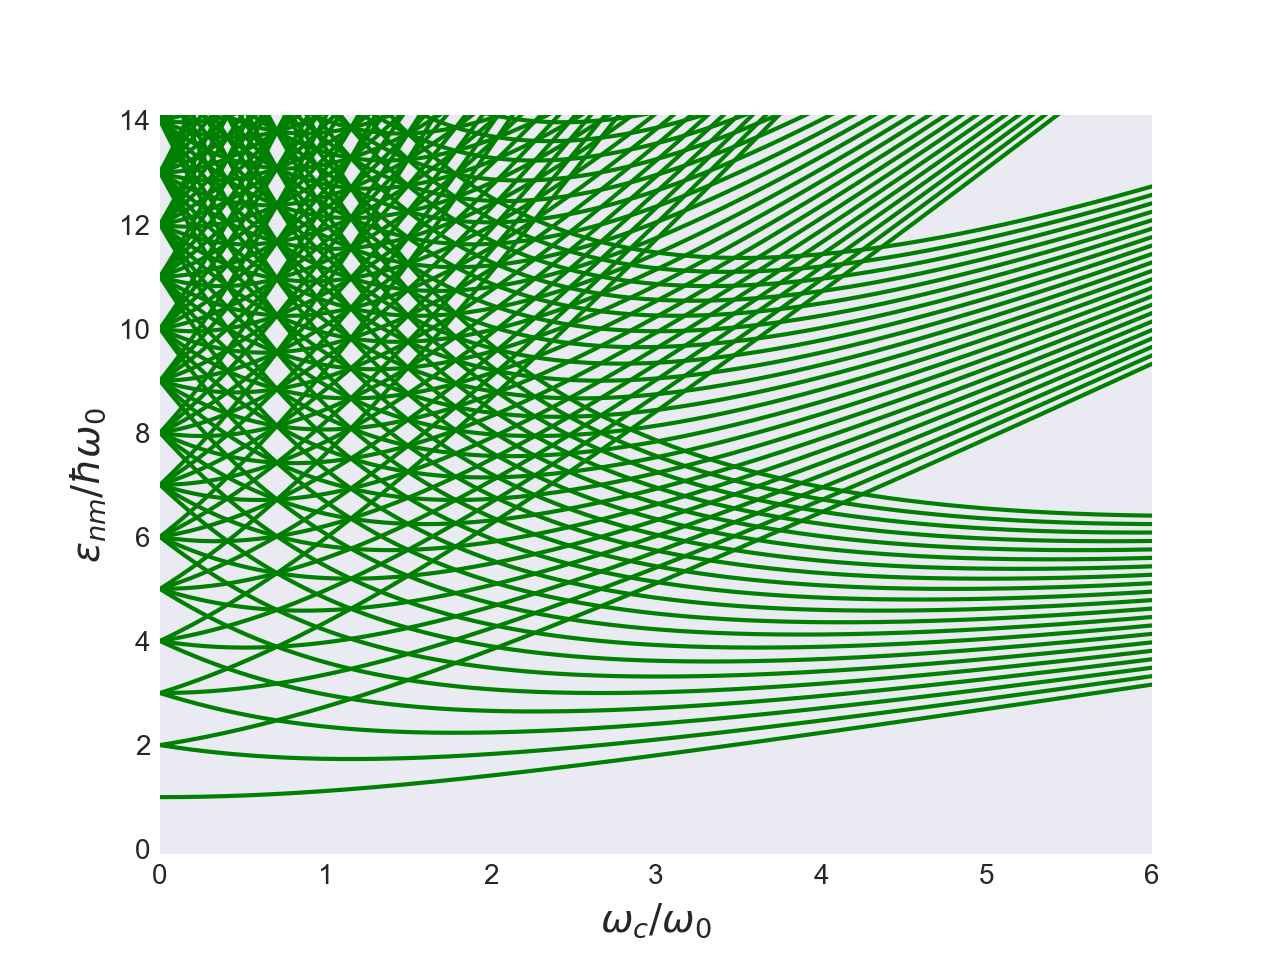
\includegraphics[width=0.75\textwidth]{implementation/figures/spaghetti.png}
    \caption{A few of the lowest eigenvalues $\epsilon_{nm}$ for a two-dimensional 
    quantum dot for transverse magnetic field of increasing strength. This plot of 
    the single-particle energies form the Fock-Darwin spectrum. Some states for very 
    high values of $m$ are omitted to make the formation of Landau bands in strong
    fields more visible.
    \label{fig:magnetic_spaghetti}}
\end{figure}

Notice in \autoref{fig:magnetic_spaghetti}, that there are lengthy intervals of 
$b$-field strength where there is no degeneracy in the eigenenergies. Conversely, 
for certain specific field strengths there are very interesting shell structures with 
diverse energies and new degeneracies. Such accidental bunching occurs 
for $\omega_c/\omega=1/\sqrt{2}, 2/\sqrt{3}, 3/2, 4/\sqrt{5}\dots$.
We also see from figure 
\autoref{fig:magnetic_spaghetti} that for an infinitely strong magnetic field as 
$\omega_c/\omega \to \infty$, in the free particle limit, that the energy levels 
form a sequence of so-called Landau bands. 

%\begin{figure}
%    \centering
%    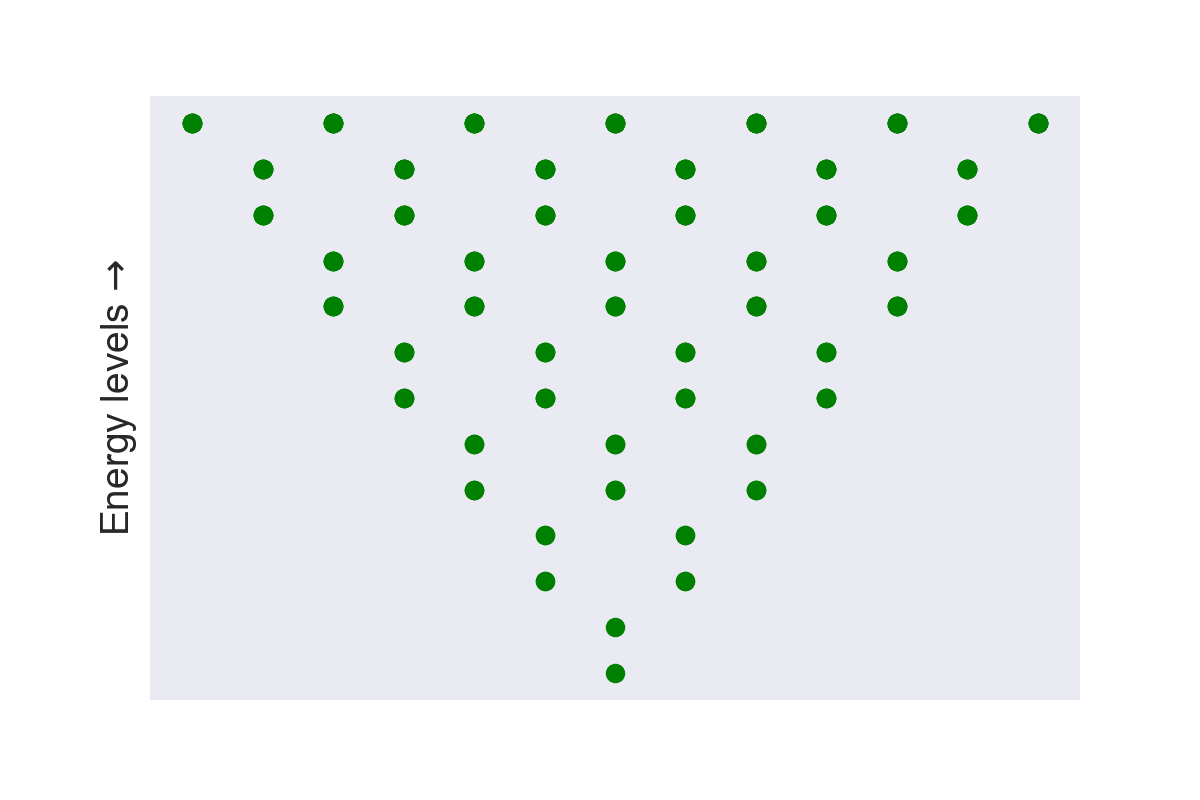
\includegraphics[width=0.75\textwidth]{implementation/figures/omega_inv_square_root_2_degeneracy.png}
%    \caption{Illustration of eigenenergy degeneracies for two-dimensional quantum 
%    dot for transverse magnetic field of strength $\omega_c=1/\sqrt{2}$.
%    Each dot 
%    \label{fig:b_field_degeneracy}}
%\end{figure}

As for the computation of the basis set, not much needs to be added in the computation 
than the extra energy to the diagonal part of the one-body matrix elements $h^p_q$, as 
everything else is the same, including the two-body Coulomb integrals. But, as we have 
already mentioned and displayed in \autoref{fig:magnetic_spaghetti}, for increasing 
strength of the magnetic field, the eigenenergies as function  of $\omega_c$ eventually 
cross over one another. The magnetic field has the effect of decreasing the energy of
a state with $m>0$ and increasing the energy of a state with $m<0$. This means that 
it is necessary to sort the eigenvalues after they have been computed. 

\section{Constructing a Custom System}

\begin{figure}
\begin{tcolorbox}
    {\fontfamily{cmss}\selectfont
    \textbf{class} quantum\_systems.\textbf{CustomSystem}

    \vspace{1em} 
    Constructs custom quantum system, where a uses can add matrix elements
    for other sources. The purpose of this class is to allow usage of 
    quantum many-body solvers that function with \emph{quantum\_systems} 
    module using other sources basis sets.

    \vspace{1em}
    \textbf{Methods:}

    \hspace{2em} \textbf{set\_h}(\emph{h}, \emph{add\_spin=False})
    \begin{adjustwidth}{4em}{}
        Add one-body matrix elements, i.e. matrix elements from non-interacting 
        part of Hamiltonian.

        \textbf{Parameters:}

        \hspace{1.5em} \textbf{h} (\emph{np.array}) One-body matrix

        \hspace{1.5em} \textbf{add\_spin} (\emph{bool}) Enforces spin orthogonality

    \end{adjustwidth}

    \hspace{2em} \textbf{set\_u}
        (\emph{u}, \emph{add\_spin=False}, \emph{anti\_symmetrize=False})
    \begin{adjustwidth}{4em}{}
        Add two-body matrix elements, i.e. matrix elements from interacting 
        part of Hamiltonian.

        \textbf{Parameters:}

        \hspace{1.5em} \textbf{u} (\emph{np.array}) Two-body matrix

        \hspace{1.5em} \textbf{add\_spin} (\emph{bool}) Enforces spin orthogonality

        \hspace{1.5em} \textbf{anti\_symmetrize} (\emph{bool})
            Anti-symmetrises two-body matrix

    \end{adjustwidth}

    \hspace{2em} \textbf{set\_s}(\emph{u}, \emph{add\_spin=False})
    \begin{adjustwidth}{4em}{}
        Add overlap matrix

        \textbf{Parameters:}

        \hspace{1.5em} \textbf{s} (\emph{np.array}) Overlap matrix

        \hspace{1.5em} \textbf{add\_spin} (\emph{bool}) Enforces spin orthogonality

    \end{adjustwidth}   

    \hspace{2em} \textbf{set\_dipole\_moment}(\emph{dipole\_moment}, \emph{add\_spin=False})
    \begin{adjustwidth}{4em}{}
        Add dipole moment, i.e. transition matrix.

        \textbf{Parameters:}

        \hspace{1.5em} \textbf{dipole\_moment} (\emph{np.array}) Dipole moment

        \hspace{1.5em} \textbf{add\_spin} (\emph{bool}) Enforces spin orthogonality

    \end{adjustwidth}

    \hspace{2em} \textbf{set\_spf}(\emph{spf}, \emph{add\_spin=False})
    \begin{adjustwidth}{4em}{}
        Add single-particle functions, i.e. eigenfunctions of non-interacting 
        part of Hamiltonian.

        \textbf{Parameters:}

        \hspace{1.5em} \textbf{spf} (\emph{np.array}) Single-particle functions

        \hspace{1.5em} \textbf{add\_spin} (\emph{bool}) Enforces spin orthogonality

    \end{adjustwidth}

    \hspace{2em} \textbf{set\_nuclear\_repulsion\_energy}
        (\emph{set\_nuclear\_repulsion\_energy})
    \begin{adjustwidth}{4em}{}
        Add nuclear repulsion energy. For atoms and molecules.

        \textbf{Parameters:}

        \hspace{1.5em} \textbf{nuclear\_repulsion\_energy} 
            (\emph{float}) Nuclear reulsion energy 

    \end{adjustwidth}


    }
\end{tcolorbox}
\end{figure}

We have constructed a subclass of the \lstinline{QuantumSystem} base 
class called \lstinline{CustomSystem} with the intent of interfacing with 
other quantum chemistry libraries. This interfacing allows us to extract basis 
sets for other systems, like atoms and molecules, that will function with the
coupled cluster solvers we have implemented.

The function of the member methods in the \lstinline{CustomSystem} class
should be evident from their names. One can set the one-body matrix elements with 
\lstinline{set_h(h, add_spin)}, set dipole matrix with 
\lstinline{set_dipole_moment(dipole_moment, add_spin)} and so on. How one would go about 
getting these structures is somewhat non-trivial, at least for someone not used 
to using quantum chemistry libraries. We have therefore added functions 
to the \lstinline{quantum_systems} module that do just that. The functions \\
\indent\lstinline{quantum_systems.custom_system.construct_psi4_system()} and \\
\indent\lstinline{quantum_systems.custom_system.construct_pyscf_system()} \\
extracts the one-body matrix, Coulomb intergrals, dipole moment, overlap matrix and
nuclear repulsion from Psi4\cite{parrish2017psi4} and PySCF\cite{PYSCF}, respectively.
The functions are provided in full in \autoref{sec:custom_system_psi4} and 
\autoref{sec:custom_system_pyscf}.
We have picked Psi4 and PySCF to interface with as they seem to be widely used in the 
quantum chemistry community. Psi4 has 354 stars and 235 forks, while PySCF has 308 stars
and 175 forks on GitHub. Arguably this can be considered  widely popular considering 
the specificity of the topic.

\begin{figure}
\begin{tcolorbox}
    {\fontfamily{cmss}\selectfont
    \textbf{class} quantum\_systems.\textbf{LaserField}
    (\emph{laser\_pulse}, \emph{polarization\_vector=None})

    \vspace{1em}
    Implementation of laser field. Needs time-dependent \emph{callable}
    to function properly.

    \vspace{1em}
    \textbf{Attributes:}
    
    \hspace{2em}\textbf{is\_one\_body\_operator} 
    Always \emph{True} 
    \textbf{Type} \emph{Bool}

    \vspace{1em} 
    \textbf{Methods:}

    \hspace{2em} \textbf{h\_t}(\emph{current\_time})
        \begin{adjustwidth}{4em}{}
            Computes one-body operator as a sum of the one-body operator of the 
            system and product of \emph{laser\_pulse} parameter at current time,
            \emph{polarization\_vector} parameter and \emph{dipole\_moment} 
            attribute of system.
        \end{adjustwidth}

    }
\end{tcolorbox}
\end{figure}

\section{Time Evolution}

In order to compute the time-development of a quantum system, we add a
time-dependent term to the Hamiltonian that describes the system. The class 
\lstinline{TimeEvolution}- \lstinline{Operator}
is an abstract base class, which defines
components necessary to make such time-dependent operators. A time-dependent 
operator usually applies solely the one- or two-body part of the Hamiltonian, and 
more often just the non-interacting one-body operator. For this reason we have implemented 
abstract attributes in the \lstinline{TimeEvolution}- \lstinline{Operator}
which will make it 
possible for the time-dependent coupled cluster solver to determine what parts 
of the Hamiltonian is necessary to update for each time step.

A common time evolution operator used in the study is a dipole approximation of 
a laser field. We have implemented a class \lstinline{LaserField}, which makes 
a simulation of such a field possible. This is a relatively simple time evolution 
operator, as it only affects the one-body part of the Hamiltonian, i.e. the 
non-interacting part. Consequently, the \lstinline{LaserField} class only needs 
to switch the \lstinline{is_one_body_operator} to \lstinline{True} and implement 
the method \lstinline{h_t(current_time)}. The time-dependent pulse, incorporating the 
shape and frequency of the laser is passed as a parameter to the class. This can be 
any callable type. The polarisation of the field is also passed to the class 
as a simple static vector, meaning that as of now the class only allows for 
linear polarisation. 
The electric field in the dipole approximation typically 
reads
\begin{equation}
    \vb{E}(t) = \vb{\epsilon} \vb{E}_0(t)\cos{(\omega t)},
\end{equation}
where $\vb{\epsilon}$ is the polarisation vector, $\vb{E}_0(t)$ defines a time-dependent 
envelope of the laser pulse, the cosine term makes sure the laser pulse is
a waveform and
$\omega$ is the angular frequency of the laser light.

\begin{figure}    
\begin{tcolorbox}
    {\fontfamily{cmss}\selectfont
    \textbf{class} quantum\_systems.\textbf{TimeEvolutionOperator}

    \vspace{1em}
    Abstract base class for time evolution operator 

    \vspace{1em}
    \textbf{Attributes:}

    \hspace{2em} \textbf{is\_one\_body\_operator} 
    \begin{adjustwidth}{4em}{}
        Property used to determine if the time-evolution operator only applies
        to the one-body part of the Hamiltonian.

        \textbf{Type} \emph{bool}       
    \end{adjustwidth}

    \hspace{2em} \textbf{is\_two\_body\_operator}
    \begin{adjustwidth}{4em}{}
        Property used to determine if the time-evolution operator only applies
        to the two-body part of the Hamiltionian.

        \textbf{Type} \emph{bool}
    \end{adjustwidth}

    \vspace{1em}
    \textbf{Methods:}

    \hspace{2em} \textbf{set\_system}(\emph{system})
    \begin{adjustwidth}{4em}{}
        Internal function used to set callback system. This is done in 
        the \emph{QuantumSystem} class and allows the user to specify 
        the time-evolution operator parameters when setting the 
        operator.

        \textbf{Parameters:}

        \hspace{1.5em} \textbf{system} (\emph{QuantumSystem}) 
            System the time-evolution operator is applied to.

    \end{adjustwidth}

    \hspace{2em} \textbf{h\_t}(\emph{current\_time})
    \begin{adjustwidth}{4em}{}
        Function computing the one-body part of the Hamiltonian for a 
        specified time.

        \textbf{Parameters:}

        \hspace{1.5em} \textbf{current\_time} (\emph{float})
            One-body operator evaluated at specified time.

        \textbf{Returns:} One-body operator.

        \textbf{Return type:} np.array
    \end{adjustwidth}

    \hspace{2em} \textbf{u\_t}(\emph{current\_time})
    \begin{adjustwidth}{4em}{}
        Function computing the two-body part of the Hamiltonian for a 
        specified time.

        \textbf{Parameters:}

        \hspace{1.5em} \textbf{current\_time} (\emph{float})
            Two-body operator evaluated at specified time.

        \textbf{Returns:} Two-body operator.

        \textbf{Return type:} np.array
    \end{adjustwidth}

    }
\end{tcolorbox}
\end{figure}
